\chapter{Load-Flow Calculation}

\section{Problem Formulation}

The aim of an load-flow analysis is to determine the voltages in the power net. Any further information, like currents in connections, critically low voltages, etc. can be derived from this result. Therefore I will consider the problem to be solved if the voltages are known.

The first step in a load flow analysis is the modelling of the net elements, as it is way to complex to use a detailed description of for instance a power plant like \figref{power_plant}. Therefore, all elements in a power net are modelled through busses, also called nodes, and admittances between them. To simplify the calculations only single phase nets are considered, therefore three phase systems have to scaled down by the factor 3, respective $\sqrt{3}$. In the model also exists only one voltage level, which means that all admittances, powers and voltages have to be scaled according to this.

The second step is then the actual calculation of the node voltages, which based is on a nodal analysis. As a pure nodal analysis is only capable of current loads it is extended to support more realistic load models.

\begin{figure}
	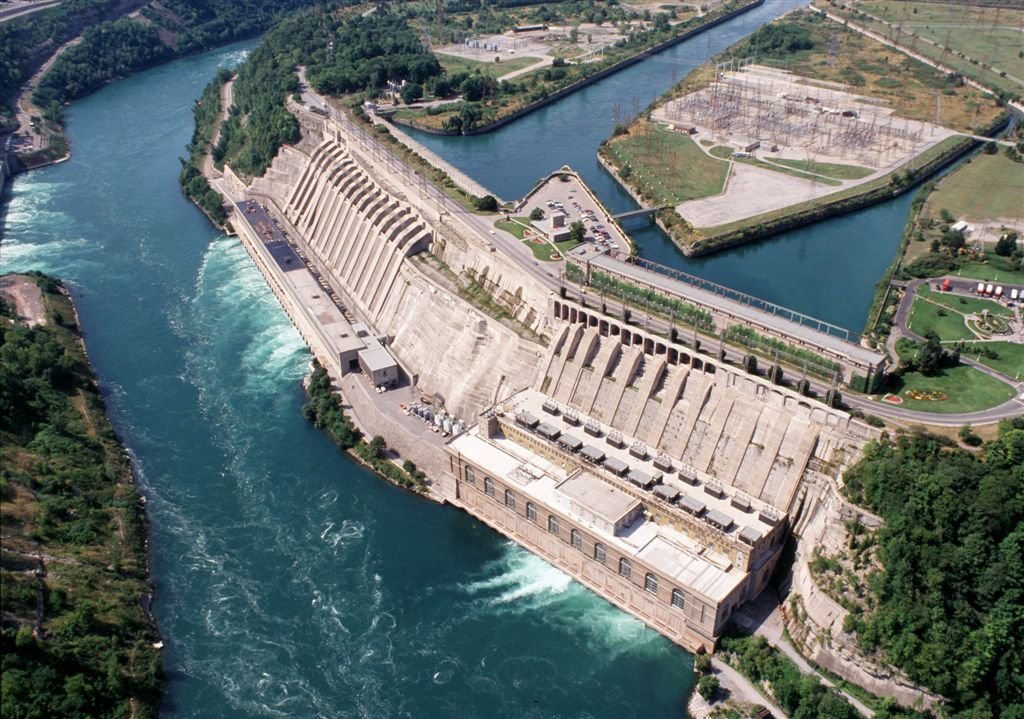
\includegraphics[width=\textwidth]{figures/adam_beck_complex.jpg}
	\caption{Sir Adam Beck Hydroelectric Generating Stations \citep{adam_back_complex}}
	\label{fig:power_plant}
\end{figure}

\subsection{Busses}

The most basic mathematical description of a an electric circuit, which an power net is, would be through admittances $Y_{ik}$ between the nodes $i$ and $k$, node voltages $U_k$ and branch currents $I_k$. In this case the element-based formulation
\begin{equation}
	\sum_i Y_{ik} U_i = I_k,
	\label{eq:current_controlled}
\end{equation}
will be used. If the loads and inputs would be current-controlled we could already stop at this point, solve the equation system and receive the node voltages as result. Unfortunately, most elements in a power net are defined through power, which is fed in, and load, which is drawn from the power net. Therefore, we have to extend \eqref{current_controlled} with a term for a constant power $S_k = P_k + j Q_k = U_k I_k^\star$ at the node $k$ and receive
\begin{equation}
	\sum_i Y_{ik} U_i = I_k + \frac{S_k^\star}{U_k^\star}.
	\label{eq:pq_bus}
\end{equation}
This formula is already the definition of a so-called PQ-bus, as at the node the real and reactive power is the defined.
Another type of bus is a slack bus. At this bus the voltage is defined, therefore we do not need any further description of this bus, but the bus is also part from neighbour busses through the branch currents $Y_{ik} U_i$. In this case, if one of the branch currents is already known, this value can be moved to the right hand side of the equation \eqref{pq_bus} and combined with $I_k$. Although, slack busses show up only in the constant currents of the right hand sides, there must be always at least one slack bus in the power net, as this bus then defines the rotation of the system and compensates mismatches in the total power sum. In practice, typically a major power plant is selected as slack bus.
The third important type of bus, beside the slack bus and PQ-bus, is the PV-bus. This is already some sort of control, as at such a node the real power $P_k$ and the voltage magnitude $|U_k|$ is defined. The implementation of this bus type depends on the algorithm which is used to calculate the missing node voltages, therefore I will discuss this in the section about the algorithms.

\subsection{Admittance Matrix}

The admittance matrix $\mat Y = (Y_{ik})$ is filled with the admittances between the nodes. More complex elements, like controlled sources, actually have to be voltage controlled, so that they can be modelled with an admittance matrix. Fortunately, most elements, which are not voltage controlled, can be transformed through a gyrator, which itself can be modelled through voltage controlled elements.

As during the modelling later several kinds of electric elements are used I will describe for each of them how they effect the admittance matrix. Each circuit element is there defined through a partial admittance matrix $\mat Y_p$, which have to be summed up afterwards to get the total admittance matrix $\mat Y$:
\begin{equation}
	\mat Y = \sum_i \mat Y_{p,i}
\end{equation}

The same superposition applies also for the current sources, if there are any.
\begin{equation}
	\vec I = \sum_i \vec I_{p,i}
\end{equation}

The two most important elements are the admittance, which is part of nearly every model of a net element, and the ideal transformer, which is mainly used for modelling real transformers which non-nominal ratios. The controlled source and the gyrator are actually only used to model the ideal transformer, which is build upon these elements.

\subsubsection{Admittance}

\begin{figure}
	\centering
	\begin{circuitikz}
	\draw (0, 0) node[left] {$U_\alpha$} to [R=$G$,o-o] (3, 0) node[right] {$U_\beta$};
\end{circuitikz} 

	\caption{Admittance $G$ between the nodes $\alpha$ and $\beta$}
	\label{fig:admittance}
\end{figure}

The admittance $G$ between the nodes $\alpha$ and $\beta$ \figref{admittance} causes the currents
\begin{equation}
	I_\alpha = (U_{k,\alpha} - U_{k,\beta}) G
\end{equation}
and
\begin{equation}
	I_\beta = (U_{k,\beta} - U_{k,\alpha}) G,
\end{equation}
which have to be considered in the admittance matrix through
\begin{equation}
	\mat Y_p = 	
	\begin{blockarray}{cccccc}
		\begin{block}{[ccccc]c}
		 		& \vdots	&			& \vdots	&			& \\
		\cdots	& G			& \cdots	& -G		& \cdots	& \alpha \\
		 		& \vdots	&			& \vdots	&			& \\
		\cdots	& -G		& \cdots	& G			& \cdots	& \beta \\
		 		& \vdots	&			& \vdots	&			& \\
		\end{block}
				& \alpha	&			& \beta		&			& 
	\end{blockarray}
\end{equation}

\subsubsection{Voltage Controlled Current Source}

\begin{figure}
	\centering
	\begin{circuitikz}
	\draw (0, 0) node[left] {$U_\delta$} to[open,o-o,v^=$u_{in}$] (0, 4) node[left] {$U_\gamma$};
	\draw (3, 4) to[european controlled current source,i=$g_m u_{in}$] (3, 0);
	\draw (3, 4) to[short,-o] (4, 4) node[right] {$U_\alpha$};
	\draw (3, 0) to[short,-o] (4, 0) node[right] {$U_\beta$};
\end{circuitikz} 

	\caption{Voltage controlled current source}
	\label{fig:voltage_controlled_current_source}
\end{figure}

The voltage controlled current source (VCCS) is again defined through the two branch currents
\begin{equation}
	I_\alpha = (U_{k,\gamma} - U_{k,\delta}) g_m
\end{equation}
and
\begin{equation}
	I_\beta = (U_{k,\delta} - U_{k,\gamma}) g_m,
\end{equation}
but with the difference to the admittance that this time the current is controlled by different nodes.

\begin{equation}
	\mat Y_p = 	
	\begin{blockarray}{cccccc}
		\begin{block}{[ccccc]c}
		 		& \vdots	&			& \vdots	&			& \\
		\cdots	& g_m		& \cdots	& -g_m		& \cdots	& \alpha \\
		 		& \vdots	&			& \vdots	&			& \\
		\cdots	& -g_m		& \cdots	& g_m		& \cdots	& \beta \\
		 		& \vdots	&			& \vdots	&			& \\
		\end{block}
				& \gamma	&			& \delta	&			& 
	\end{blockarray}
\end{equation}

\subsubsection{Gyrator}

\begin{figure}
	\centering
	\begin{circuitikz}
	\draw (0, 0) node[gyrator] (G) {};
	\draw (G.base) node{$G_D$};
  	\draw ($(G.A1) - (1, 0)$) node[left] {$U_\alpha$} to[short,o-,i=$i_1$] (G.A1);
  	\draw (G.A2) to[short,-o] ($(G.A2) - (1, 0)$) node[left] {$U_\beta$};
  	\draw ($(G.B1) + (1, 0)$) node[right] {$U_\gamma$} to[short,o-,i=$i_2$] (G.B1);
  	\draw (G.B2) to[short,-o] ($(G.B2) + (1, 0)$) node[right] {$U_\delta$};
  	\draw ($(G.A2) - (1, 0)$) to[open,v^=$u_1$] ($(G.A1) - (1, 0)$);
  	\draw ($(G.B2) + (1, 0)$) to[open,v=$u_2$] ($(G.B1) + (1, 0)$);
\end{circuitikz}
	\caption{Gyrator}
	\label{fig:gyrator_original}
\end{figure}

\begin{figure}
	\centering
	\begin{circuitikz}	
	\draw (1, 2.5) to[european controlled current source,i_=$G_D u_2$] (1, 0);
	\draw (-1, 2.5) node[left] {$U_\alpha$} to[short,i=$i_1$,o-] (1, 2.5);
	\draw (1, 0) to[short,-o] (-1, 0) node[left] {$U_\beta$};
	\draw (-1, 0) to[open,v^=$u_1$] (-1, 2.5);
	\draw (3, 2.5) to[european controlled current source,i=$-G_D u_1$] (3, 0);
	\draw (5, 2.5) node[right] {$U_\gamma$} to[short,i=$i_2$,o-] (3, 2.5);
	\draw (3, 0) to[short,-o] (5, 0) node[right] {$U_\delta$};
	\draw (5, 0) to[open,v=$u_2$] (5, 2.5);
\end{circuitikz} 

	\caption{Equivalent circuit for a gyrator}
	\label{fig:gyrator_equivalent}
\end{figure}

The gyrator \figref{gyrator_original}, which is defined by
\begin{equation}
	i_1 = G_D u_2
\end{equation}
and
\begin{equation}
	i_2 = -G_D u_1
\end{equation}
can be replaced with two VCCSs like in \figref{gyrator_equivalent}.

\subsubsection{Ideal Transformer}

\begin{figure}
	\centering
	\begin{circuitikz}
	\draw (0, 0) node[transformer core] (T) {};
	\draw ($(T.base) + (0, 0.3)$) node{$a : 1$};
  	\draw ($(T.A1) - (1, 0)$) node[left] {$U_\alpha$} to[short,o-,i=$i_1$] (T.A1);
  	\draw (T.A2) to[short,-o] ($(T.A2) - (1, 0)$) node[left] {$U_\beta$};
  	\draw ($(T.B1) + (1, 0)$) node[right] {$U_\gamma$} to[short,o-,i=$i_2$] (T.B1);
  	\draw (T.B2) to[short,-o] ($(T.B2) + (1, 0)$) node[right] {$U_\delta$};
  	\draw ($(T.A2) - (1, 0)$) to[open,v^=$u_1$] ($(T.A1) - (1, 0)$);
  	\draw ($(T.B2) + (1, 0)$) to[open,v=$u_2$] ($(T.B1) + (1, 0)$);
\end{circuitikz}
	\caption{Ideal transformer}
	\label{fig:ideal_transformer_original}
\end{figure}

\begin{figure}
	\centering
	\begin{circuitikz}
	\draw (0, 0) node[gyrator] (G1) {};
	\draw (2, 0) node[gyrator] (G2) {};
	\draw (G1.base) node{$a R$};
	\draw (G2.base) node{$R$};
	\draw (G1.B1) to[short,-*] (G1.B1) node[above] {$U_\epsilon$};
  	\draw ($(G1.A1) - (0.5, 0)$) node[left] {$U_\alpha$} to[short,o-,i=$i_1$] (G1.A1);
  	\draw (G1.A2) to[short,-o] ($(G1.A2) - (0.5, 0)$) node[left] {$U_\beta$};
  	\draw ($(G2.B1) + (0.5, 0)$) node[right] {$U_\gamma$} to[short,o-,i=$i_2$] (G2.B1);
  	\draw (G2.B2) to[short,-o] ($(G2.B2) + (0.5, 0)$) node[right] {$U_\delta$};
  	\draw ($(G1.A2) - (0.5, 0)$) to[open,v^=$u_1$] ($(G1.A1) - (0.5, 0)$);
  	\draw ($(G2.B2) + (0.5, 0)$) to[open,v=$u_2$] ($(G2.B1) + (0.5, 0)$);
  	\draw (G1.A2) to[short] (G1.B2);
\end{circuitikz}
	\caption{Equivalent circuit for an ideal transformer}
	\label{fig:ideal_transformer_equivalent}
\end{figure}

An ideal transformer like in \figref{ideal_transformer_original} is modelled with two gyrators according to the circuit \figref{ideal_transformer_equivalent}. The gyrators themselves have to be replaced by voltage controlled elements, like it was presented previously.

The parameter $R$ in this model can be chosen freely in theory, but for numerical reasons I recommend such a scaling of the internal node, that it is in the range of the nominal voltages. To be able to do this an estimation of the load flow over the transformer is needed, but it is sufficient to have a very rough estimate. If the scaling is chosen improperly especially the iterative methods to solve the load flow problem will not convergence in most cases.

\section{Scaling}

As long as the relations are kept the same it is possible to change the scale base of all values in a system. For purpose from the set of voltage, current, impedance and power two physical quantities can be freely chosen and the others arise out of this decision. Another term for this scaling is the transformation into a so-called per-unit system \citep[p. 90]{powerSystemAnalysis}.

For numerical stability the voltages should be in the range of 1, therefore for each voltage level in the system the nominal voltage is selected as scale base $U_B$ for the voltages. The degree of freedom can be used to scale also the powers down into the range of 1, which can be achieved for instance roughly with the scale base
\begin{equation}
	P_B = \frac{1}{2n} \left( \sum_{i}^n \left| P_{load,i} \right| + \sum_{i}^n \left| Q_{load,i} \right| \right)
\end{equation}
for the powers. 

The other scale bases are then derived from these two chosen values:
\begin{equation}
	I_B = \frac{P_B}{U_B}
\end{equation}
\begin{equation}
	Z_B = \frac{1}{Y_B} = \frac{U_B}{I_B}
\end{equation}

The actually scaling is achieved through a division of the values by the scale bases.
\begin{equation}
	U_{scaled} = \frac{U}{U_B}
\end{equation}
\begin{equation}
	I_{scaled} = \frac{I}{I_B}
\end{equation}
\begin{equation}
	P_{scaled} = \frac{P}{P_B}
\end{equation}
\begin{equation}
	Q_{scaled} = \frac{Q}{P_B}
\end{equation}
\begin{equation}
	Z_{scaled} = \frac{Z}{Z_B}
\end{equation}
\begin{equation}
	Y_{scaled} = \frac{Y}{Y_B}
	\label{eq:scaling_admittance}
\end{equation}

\section{Modelling of Net Elements}

The power net elements are modelled through admittances and busses, therefore we will use the previously derived knowledge to describe the behaviour of the net elements.

All external nodes which exist in a power net are by default PQ-busses with no load, therefore $P = 0$ and $Q = 0$. The direct combination of PQ-busses leads to a summation of the partial inputs (or loads, depending on the sign). The direct connection of a PV-bus to a PQ-bus instead has the result, that bus is forced to become a PV-bus with the values $P_{total} = P_{PV} + P_{PQ}$ and $V_{total} = V_{PV}$. The reactive power of the PQ-node is assumed to be provided by the PV-bus. The third type of busses, a slack bus, can be combined with a PQ-bus too. In this case all loads are provided by the slack bus itself, therefore the total result is a slack bus.

As it would lead to an overspecified problem PV-busses must not be connected to slack busses. Theoretically this is possible if the PV-bus has the same voltage magnitude as the slack bus, but in practice this case does not occur and can be neglected.

\subsection{Transmission Line}
A transmission line is modelled only with admittances like in \figref{transmission_line}. The values $Y_q$ and $Y_l$ can be derived from the wave impedance $Z_W$, the propagation constant $\gamma$ and the length of the transmission line through
\begin{equation}
	Y_l = \frac{1}{Z_W \sinh \left( \gamma l \right)}
\end{equation}
and
\begin{equation}
	\frac{Y_q}{2} = \frac{1}{Z_W} \tanh \left( \frac{\gamma l}{2} \right),
\end{equation}
as shown in \citep[p. 155]{powerSystemAnalysis}. The wave impedance and the propagation constant can be calculated from the electrical characteristics with
\begin{equation}
	Z_W = \sqrt{\frac{R' + j \omega L'}{G' + j \omega C}}
\end{equation}
and 
\begin{equation}
	\gamma = \sqrt{\left( R' + j \omega L' \right) \left( G' + j \omega C \right)},
\end{equation}
also derived in \citep[p. 153]{powerSystemAnalysis}.

\begin{figure}
	\centering
	\begin{circuitikz}
	\draw (1, 0) to [R=$\frac{Y_{q}}{2}$,*-*] (1, 2.5);
	\draw (1, 2.5) to [R=$Y_{l}$,*-*] (3.5, 2.5);
	\draw (3.5, 0) to [R=$\frac{Y_{q}}{2}$,*-*] (3.5, 2.5);
	\draw (1, 0) to (3.5, 0);
	\draw (0, 0) to [short,o-*] (1, 0);
	\draw (0, 2.5) to [short,o-*] (1, 2.5);
	\draw (3.5, 0) to [short,*-o] (4.5, 0);
	\draw (3.5, 2.5) to [short,*-o] (4.5, 2.5);
	\draw (1, 0) to (1, -0.25) node[ground] {};
	\draw (0, 0) to [open,v^=$U_i$] (0, 2.5);
	\draw (4.5, 0) to [open,v=$U_j$] (4.5, 2.5);
\end{circuitikz} 

	\caption{Equivalent circuit for a transmission line}
	\label{fig:transmission_line}
\end{figure}

\subsection{Load}
A load can be modelled through a PQ-bus and no change to the admittance matrix. If there are several loads connected to one node their values sum up as already discussed before.

\subsection{Generator}

\begin{figure}
	\centering
	\begin{circuitikz}
	\draw (0, 0) node[below] {$|U| = E$, $P = P_{in}$} to [R=$jX_d$,*-o] (4, 0) node[above] {$U_\alpha$};
\end{circuitikz} 

	\caption{Equivalent circuit for a generator}
	\label{fig:generator}
\end{figure}

Generators are represented through a synchronous reactance $X_d$, which models internal losses, and a PV-bus \citep[p. 55]{powerSystemAnalysis}, like it can be seen in \figref{generator}. The voltage magnitude at the internal PV-bus is the excitation voltage $E$ and the real power input is determined by the mechanical power and some transformation losses. 

If the synchronous reactance is not zero the external node $\alpha$ is not forced to any certain bus type, but if it is zero, the bus is forced to become a PV-bus.

\subsection{Transformer}

\begin{figure}
	\centering
	\begin{circuitikz}
	\draw (0, 0) node[transformer core] (T) {};
	\draw ($(T.base) + (0, 0.3)$) node{$a : 1$};
  	\draw (T.A1) to[short] ($(T.A1) - (0.5, 0)$);
  	\draw (T.A2) to[short] ($(T.A2) - (0.5, 0)$);
  	\draw ($(T.A2) - (0.5, 0)$) to[R=$Y_q$,*-*] ($(T.A1) - (0.5, 0)$);
  	\draw ($(T.A1) - (3, 0)$) to[R=$Y_l$,*-*] ($(T.A1) - (0.5, 0)$);
  	\draw ($(T.A1) - (3, 0)$) to[R=$Y_q$,*-*] ($(T.A2) - (3, 0)$);
  	\draw ($(T.A2) - (0.5, 0)$) to[short] ($(T.A2) - (3, 0)$);
  	\draw ($(T.B1) + (1, 0)$) to[short,o-,i=$I_2$] (T.B1);
  	\draw (T.B2) to[short,-o] ($(T.B2) + (1, 0)$);
  	\draw ($(T.A1) - (4, 0)$) to[short,o-,i=$I_1$] ($(T.A1) - (3, 0)$);
  	\draw ($(T.A2) - (4, 0)$) to[short,o-] ($(T.A2) - (3, 0)$);
  	\draw ($(T.A2) - (4, 0)$) to[open,v^=$U_1$] ($(T.A1) - (4, 0)$);
  	\draw ($(T.B2) + (1, 0)$) to[open,v=$U_2$] ($(T.B1) + (1, 0)$);
\end{circuitikz}
	\caption{Equivalent circuit for a transformer}
	\label{fig:transformer}
\end{figure}

To model the transformer I chose to use the equivalent circuit \figref{transformer} with a $\pi$-model and an ideal transformer. As all variables are scaled to the same nominal voltage the ideal transformer is only needed, if the real transmission ratio $a$ is not the nominal transmission ratio
\begin{equation}
	a_n = \frac{U_{1n}}{U_{2n}}.
\end{equation}
In this case the ratio of the ideal transformer is set to the relative ratio
\begin{equation}
	a_r = \frac{a}{a_n}.
\end{equation}
For transformer exist several different ways to specifiy their electrical characeristics. I've chosen to use as input:
\begin{itemize}
	\item $S_n$: nominal power
	\item $|u_r|$: relative short circuit voltage
	\item $P_{Cu}$: copper losses
	\item $P_{Fe}$: iron losses
	\item $\frac{I_0}{I_n}$: relative no-load current
\end{itemize}

The shunt admittance can then be derived direct from these values through
\begin{equation}
	Y_q = \frac{1}{2} \left( P_{Fe} - j \frac{I_0}{I_n} S_n \right) \frac{1}{U_{2n}^2}.
\end{equation}

For the length admittance it is first necessary to calculate the complex relative short circuit voltage $u_r$. The real part
\begin{equation}
	\Re{u_r} = \frac{P_{Cu}}{S_n}
\end{equation}
can be calculate from the copper losses and the nominal power. As now the magnitude and the real part of the relative short circuit voltage are known, it is possible to calculate the imaginary part
\begin{equation}
	\Im{u_r} = \sqrt{|u_r|^2 - \Re{u_r}}.
\end{equation}
Therefore, the total complex short circuit voltage
\begin{equation}
	u_r = \Re{u_r} + j \Im{u_r}
\end{equation}
is known too and the length admittance
\begin{equation}
	Y_l = \frac{S_n}{U_{1n}^2 u_r}
\end{equation}
can be calculated.

Before these admittances are inserted into the admittance matrix they have to be scaled according to \eqref{scaling_admittance}.

\subsection{Feed-In}

\begin{figure}
	\centering
	\begin{circuitikz}
	\draw (0, 0) node[above] {$U_{slack}$} to [R=$Z_q$,*-o] (4, 0) node[above] {$U$};
\end{circuitikz} 

	\caption{Equivalent circuit for a feed-in}
	\label{fig:feedin}
\end{figure}

A feed-in \figref{feedin} is characterized through the voltage at the internal slack bus $U_{slack}$, the short circuit power $S_k$, the power factor $c$ and the ratio of the real to the imaginary part $\frac{R}{X}$. From these values the magnitude of the input impedance 
\begin{equation}
	|Z_q| = c \frac{U_n}{S_k}
\end{equation}
can be derived, which therefore is the enables the calculation of
\begin{equation}
	X = \frac{\sqrt{\left( \frac{R}{X} \right) + 1}}{|Z_q|}
\end{equation}
and
\begin{equation}
	R = \frac{R}{X} \cdot X.
\end{equation}
These two values combined are then the input impedance
\begin{equation}
	Z_q = R + j X.
\end{equation}

In case the short circuit power is very high compared to the actual load flow the input impedance may turn out to have a very small value, which could be neglected. This results then in a direct connection of the internal slack bus with the external node. Therefore, the external node is overriden and turns into a slack bus.

\section{Calculation Methods}

The task for the following calculation methods is to determine the node voltages from a admittance matrix, a list of PQ- and PV-busses and a vector of constant currents. In this section I will describe in total four different algorithms for this problem:
\begin{itemize}
	\item Current Iteration \citep[p. 209]{powerSystemAnalysis}
	\item Newton-Raphson \citep[p. 232]{powerSystemAnalysis}
	\item Fast-decoupled-load-flow \citep[p. 240]{powerSystemAnalysis}
	\item Holomorphic Embedding Load Flow \citep{helmIEEE, helmPatentApr2009, helmPatentSept2009}
\end{itemize}

As short overview I will start with a classification of these methods, based on their specific characteristics.

\subsection{Classification of Methods}

The first three methods, Current Iteration, Newton-Raphson and the FDLF, fall into the category of iterative methods. These algorithms are well studied since centuries now, but have two major drawbacks. First of all, they are iterative and need some seed values for the voltages. And this point leads direct to the second drawback: The iterative methods can not guarantee to find a solution and their convergence depends heavily on the initial voltages. It may even happen that the iterative methods produce results which are not physical, what in this case means that they do no represent a stable operating point. This happens typically only for certain constructed power nets, but in practice the bigger problem is that these methods often do not converge, although the power net is in a stable condition.

To circumvent these drawbacks a new approach to the load flow problem was developed, the so-called Holomorphic Embedding Load Flow. This algorithm guarantees in theory to converge, if and only if, the system is stable. Therefore HELM would be superior to the iterative methods, but it has some drawbacks in practice which will be discussed in \secref{comparison_algorithms}. 

\subsection{Current Iteration}
\label{sec:current_iteration}

The basic problem of the load flow calculation is that \eqref{pq_bus} can not be solved explicitly. The iterative approach of the Current Iteration works around this problem through a selection of initial voltages and the successive solving of one line of \eqref{pq_bus} after another. To do so on the left hand side of the equation the current voltage is separated from the sum
\begin{equation}
	\sum_{i \ne k} Y_{ik} U_i + Y_{kk} U_k = I_k + \frac{S_k^\star}{U_k^\star}
\end{equation}
and then the rest is brought to the right hand side
\begin{equation}
	 U_k = \frac{1}{Y_{kk}} \left( I_k + \frac{S_k^\star}{U_k^\star} - \sum_{i \ne k} Y_{ik} U_i \right).
\end{equation}
The resulting equation is again not explicitly solved for $U_k$ as this variable still occurs on the right hand side, but at this appearance the old value, from the previous iteration, can be used. This leads then to
\begin{equation}
	 U_k^{j + 1} = \frac{1}{Y_{kk}} \left( I_k + \frac{S_k^\star}{U_k^{(j) \star}} - \sum_{i \ne k} Y_{ik} U_i^{(j)} \right),
\end{equation}
where the superindex $j$ denotes the iteration step. For the sake of legibilty with this formula one would actually update the node voltages only after every iteration, but they can actually be updated every time a new value is calculated.

To this point only the PQ-busses were discuess, but PV-busses can be handled too. For this purpose the PV-bus is considered as PQ-bus in the first step, and afterwards the values are corrected to match the needs of the PV-bus \citep[p. 211]{powerSystemAnalysis}. One possible way to calculate the updated voltage $U_k'$ is to combine the specified voltage magnitude $|U_{k,PV}|$ with the newly calculate $U_k$ like
\begin{equation}
	U_k' = |U_{k,PV}| e^{j \angle U_k}.
\end{equation}

\subsection{Newton-Raphson}
\label{sec:newton_raphson}

In general, under the name Newton-Raphson a method for finding roots of a nonlinear function is known. In the area of load flow calculation the idea is the same, the problem is transformed into finding voltages $\vec x$ so that the loads driven by these voltages $\vec S (\vec x)$ is the same as the specified loads $S_{spec}$:
\begin{equation}
	\vec S (\vec x) = S_{spec}
\end{equation}
With a small transformation this leads to the problem of finding the roots of
\begin{equation}
	\vec S (\vec x) - S_{spec} = 0,
\end{equation}
which is exactly what Newton-Raphson does. For this the whole left part is considered as function
\begin{equation}
	\vec f (\vec x) = \vec S (\vec x) - S_{spec},
\end{equation}
which is developed into the Taylor-series
\begin{equation}
	\vec f (\vec x) = \sum_{k = 0}^\infty \frac{\vec f^{(k)} (\vec x_0}{k!} \left( \vec x - \vec x_0 \right).
\end{equation}
This series is terminated after the linear term, which leads to the approximation
\begin{equation}
	\vec f (\vec x) \approx \vec f (\vec x_0) + \vec f' (\vec x_0) \left( \vec x - \vec x_0 \right).
\end{equation}

As we actually want to find the root of $\vec f (\vec x)$ we set the approximation to 0 and replace in the result
\begin{equation}
	0 = \vec f (\vec x_k) + \vec f' (\vec x_k) \left( \vec x_{k + 1} - \vec x_k \right)
\end{equation}
the occurence of $\vec f (\vec x)$ with its definition to get
\begin{equation}
	\vec S' (\vec x_k) \left( \vec x_{k + 1} - \vec x_k \right) = \vec S (\vec x_k) - \vec S_{spec}.
	\label{eq:newton_raphson_equation_system}
\end{equation}
In this formula we have on the left side as matrix the derivation of the power function with respect to the voltages $\vec S' (\vec x_k)$, the voltage changes $\Delta \vec x_k = \left( \vec x_{k + 1} - \vec x_k \right)$ and on the right side the current power mismatch 
\begin{equation}
	\Delta \vec S (\vec x_k) = \vec S (\vec x_k) - \vec S_{spec}.
	\label{eq:power_mismatch}
\end{equation}

This is then an iterative approach, where we can calculate from the current power mismatch improved voltages, calculate the power mismatch again, ... and so on. The open question at this point is how to represent the voltages, as they are complex variables. As in practice the in real power nets the voltage magnitude $|U_i|$ of a node is mainly depending on the reactive power and the angle of the voltage $\delta_i$ on the real power, the voltages are represented in polar coordinates. Therefore, in case we consider $n$ PQ-busses and $m$ PV-busses, we have as voltage vector 
\begin{equation}
	\vec x = 
	\begin{bmatrix}
		|U_1| \\
		\vdots \\
		|U_n| \\
		\delta_1 \\
		\vdots \\
		\delta_n \\
		\delta_{n + 1} \\
		\vdots \\
		\delta_{n + m} 
	\end{bmatrix} = 	
	\begin{bmatrix}
		|U_1| \\
		\vdots \\
		|U_n| \\
		\delta_1 \\
		\vdots \\
		\delta_{n + m} 
	\end{bmatrix}
\end{equation}
and for the specified powers
\begin{equation}
	\vec S_{spec} = 
	\begin{bmatrix}
		P_1 \\
		\vdots \\
		P_n \\
		P_{n + 1} \\
		\vdots \\
		P_{n + m} \\
		Q_1 \\
		\vdots \\
		Q_n
	\end{bmatrix} = 
	\begin{bmatrix}
		P_1 \\
		\vdots \\
		P_{n + m} \\
		Q_1 \\
		\vdots \\
		Q_n
	\end{bmatrix}.
\end{equation}

The last missing part is the derivation of the power function, which means we have to start to separate the power at each node into its real and imaginary part and derive these functions then with respect to the voltage magnitudes and angles.

As first step \eqref{pq_bus} is transformed into an explicit calculation of the power at the bus $k$
\begin{align}
	S_k &= \left( U_k^\star \left( \sum_{i \ne k} Y_{ik} U_i + Y_{kk} U_k - I_k \right) \right)^\star \\
		&= U_k \left( \sum_{i \ne k} Y_{ik}^\star U_i^\star + Y_{kk}^\star U_k^\star - I_k^\star \right) \\
		&= \sum_{i \ne k} U_k Y_{ik}^\star U_i^\star + Y_{kk}^\star |U_k|^2 - I_k^\star U_k.
\end{align}
Next, the variables are split up into magnitude and angle ($U_k = |U_k| e^{j \delta_k}$, $I_k = |I_k| e^{j \gamma_k}$, $Y_{ik} = |Y_{ik}| e^{j \theta_{ik}}$) which leads to the expression
\begin{align}
	S_k &= \sum_{i \ne k} |U_k| e^{j \delta_k} |Y_{ik}| e^{-j \theta_{ik}} |U_i| e^{-j \delta_i} + |Y_{kk}| e^{-j \theta_{kk}} |U_k|^2 - |I_k| e^{-j \gamma_k} |U_k| e^{j \delta_k} \\
		&= \sum_{i \ne k} |U_k| |Y_{ik}| |U_i| e^{j \left( \delta_k - \theta_{ik} - \delta_i \right)} + |Y_{kk}| |U_k|^2 e^{-j \theta_{kk}} - |I_k| |U_k| e^{j \left( \delta_k - \gamma_k \right)}
		\label{eq:newton_raphson_polar}
\end{align}
for the load at bus $k$. This load can be separated into its real and imaginary part
\begin{equation}
	S_k = P_k + j Q_k,
\end{equation}
as well as the part on the right hand side of \eqref{newton_raphson_polar} to receive
\begin{equation}
	P_k = \sum_{i \ne k} |U_k| |Y_{ik}| |U_i| \cos \left( \delta_k - \theta_{ik} - \delta_i \right) + |Y_{kk}| |U_k|^2 \cos \left( \theta_{kk} \right) - |I_k| |U_k| \cos \left( \delta_k - \gamma_k \right)
\end{equation}
and
\begin{equation}
	Q_k = \sum_{i \ne k} |U_k| |Y_{ik}| |U_i| \sin \left( \delta_k - \theta_{ik} - \delta_i \right) - |Y_{kk}| |U_k|^2 \sin \left( \theta_{kk} \right) - |I_k| |U_k| \sin \left( \delta_k - \gamma_k \right).
\end{equation}
These formulas now have to be differentiate with respect to $U_k$, $U_i$ ($i \ne k$), $\delta_k$ and $\delta_i$ ($i \ne k$):
\begin{equation}
	\frac{\partial P_k}{\partial |U_k|} = \sum_{i \ne k} |Y_{ik}| |U_i| \cos \left( \delta_k - \theta_{ik} - \delta_i \right) + 2 |Y_{kk}| |U_k| \cos \left( \theta_{kk} \right) - |I_k| \cos \left( \delta_k - \gamma_k \right)
\end{equation}
\begin{equation}
	\frac{\partial Q_k}{\partial |U_k|} = \sum_{i \ne k} |Y_{ik}| |U_i| \sin \left( \delta_k - \theta_{ik} - \delta_i \right) - 2 |Y_{kk}| |U_k| \sin \left( \theta_{kk} \right) - |I_k| \sin \left( \delta_k - \gamma_k \right)
\end{equation}
\begin{equation}
	\frac{\partial P_k}{\partial |U_i|} = |U_k| |Y_{ik}| \cos \left( \delta_k - \theta_{ik} - \delta_i \right)
\end{equation}
\begin{equation}
	\frac{\partial Q_k}{\partial |U_i|} = |U_k| |Y_{ik}| \sin \left( \delta_k - \theta_{ik} - \delta_i \right)
\end{equation}
\begin{equation}
	\frac{\partial P_k}{\partial \delta_k} = - \sum_{i \ne k} |U_k| |Y_{ik}| |U_i| \sin \left( \delta_k - \theta_{ik} - \delta_i \right) + |I_k| |U_k| \sin \left( \delta_k - \gamma_k \right)
\end{equation}
\begin{equation}
	\frac{\partial Q_k}{\partial \delta_k} = \sum_{i \ne k} |U_k| |Y_{ik}| |U_i| \cos \left( \delta_k - \theta_{ik} - \delta_i \right) - |I_k| |U_k| \cos \left( \delta_k - \gamma_k \right)
\end{equation}
\begin{equation}
	\frac{\partial P_k}{\partial \delta_i} = |U_k| |Y_{ik}| |U_i| \sin \left( \delta_k - \theta_{ik} - \delta_i \right)
\end{equation}
\begin{equation}
	\frac{\partial Q_k}{\partial \delta_i} = - |U_k| |Y_{ik}| |U_i| \cos \left( \delta_k - \theta_{ik} - \delta_i \right)
\end{equation}

With these derivations we can calculate the derivation of the power functions with form the Jacobian matrix
\begin{equation}
	\vec S' (\vec x_k) = 
	\begin{bmatrix}
		\frac{\partial P_1}{\partial |U_1|}	& \hdots	& \frac{\partial P_1}{\partial |U_n|}	& \frac{\partial P_1}{\partial \delta_1}	& \hdots	& \frac{\partial P_1}{\partial \delta_{n + m}} \\
		\vdots								&			& \vdots								& \vdots									&			& \vdots \\
		\frac{\partial P_{n + m}}{\partial |U_1|}	& \hdots	& \frac{\partial P_{n + m}}{\partial |U_n|}	& \frac{\partial P_{n + m}}{\partial \delta_1}	& \hdots	& \frac{\partial P_{n + m}}{\partial \delta_{n + m}} \\
		\frac{\partial Q_1}{\partial |U_1|}	& \hdots	& \frac{\partial Q_1}{\partial |U_n|}	& \frac{\partial Q_1}{\partial \delta_1}	& \hdots	& \frac{\partial Q_1}{\partial \delta_{n + m}} \\
		\vdots								&			& \vdots								& \vdots									&			& \vdots \\
		\frac{\partial Q_n}{\partial |U_1|}	& \hdots	& \frac{\partial Q_n}{\partial |U_n|}	& \frac{\partial Q_n}{\partial \delta_1}	& \hdots	& \frac{\partial Q_n}{\partial \delta_{n + m}}
	\end{bmatrix}.
	\label{eq:power_jacobian_newton_raphson}
\end{equation}

The iterative process to improve the voltages is then:
\begin{enumerate}
	\item Calculate the current power mismatch $\Delta \vec S (\vec x_k)$ with \eqref{power_mismatch}
	\item Calculate the Jacobian matrix $\vec S' (\vec x_k)$ with \eqref{power_jacobian_newton_raphson}
	\item Calculate the voltage changes $\Delta \vec x_k$ through solving the linear equation system \eqref{newton_raphson_equation_system}
	\item Calculate the improved voltages through $\vec x_{k + 1} = \vec x_k + \Delta \vec x_k$
	\item Repeat these steps until the voltage change is small enough
\end{enumerate}

\subsection{Fast-decoupled-load-flow}
\label{sec:fdlf}

The FDLF is a modification of the Newton-Raphson method, which is based on an observation already discussed previously. The change in voltage magnitudes is mostly driven by the reactive power flow and the change in the voltage angles by the real power flow. With this in mind one can neglect two quarters of the Jacobian matrix in \eqref{power_jacobian_newton_raphson} and reduce the matrix therefore to
\begin{equation}
	\vec S' (\vec x_k) \approx 
	\begin{bmatrix}
		0	& \hdots	& 0	& \frac{\partial P_1}{\partial \delta_1}	& \hdots	& \frac{\partial P_1}{\partial \delta_{n + m}} \\
		\vdots								&			& \vdots								& \vdots									&			& \vdots \\
		0	& \hdots	& 0	& \frac{\partial P_{n + m}}{\partial \delta_1}	& \hdots	& \frac{\partial P_{n + m}}{\partial \delta_{n + m}} \\
		\frac{\partial Q_1}{\partial |U_1|}	& \hdots	& \frac{\partial Q_1}{\partial |U_n|}	& 0	& \hdots	& 0 \\
		\vdots								&			& \vdots								& \vdots									&			& \vdots \\
		\frac{\partial Q_n}{\partial |U_1|}	& \hdots	& \frac{\partial Q_n}{\partial |U_n|}	& 0	& \hdots	& 0
	\end{bmatrix} =
	\begin{bmatrix}
		0								&	\frac{\partial P}{\partial \delta} \\
		\frac{\partial Q}{\partial |U|}	&	0
	\end{bmatrix}.
\end{equation}

With this simplified system matrix the equation system \eqref{newton_raphson_equation_system} can be seperated into
\begin{equation}
	\frac{\partial P}{\partial \delta} \cdot \Delta \delta_k = \Delta P_k
\end{equation}
and
\begin{equation}
	\frac{\partial Q}{\partial |U|} \cdot \Delta |U|_k = \Delta Q_k.
\end{equation}

The steps for solving the load flow problem are nearly the same as for the Newton-Raphson, the only difference lies within the smaller linear equation system which needs to be solved. This is already the reason why one may chose the FDLF instead of the Newton-Raphson: the calculation is faster. The disadvantage of the simplification is a worse convergence behaviour, therefore the FDLF is less probable to be actually capable of solving a load flow problem.

\subsection{Holomorphic Embedding Load Flow}
\label{sec:helm}

HELM is a comparatively young algorithm for the load flow problem, as it was developed 2012 \citep{helmIEEE}. The basic idea behind it is to replace the voltages with voltage functions and their Laurent series. Through this approach it is possible to guarantee that the algorithm will converge if, and only if, the power net is stable. With this advantage in mind I will start in this section with the theory behind HELM, the practical implications will be discussed in \secref{results}.

\subsubsection{Calculation of Coefficients}

The starting point for HELM is \eqref{pq_bus}, where the slack busses are already considered as constant currents. As already mentioned before, because of its structure it is not possible to solve this equation respectively equation system explicitly. Therefore, the voltages $U_i$ are replaced with the functions $U_i(s)$. To achieve even further that these functions are holomorph \citep{helmPatentSept2009} \eqref{pq_bus} is extended to
\begin{equation}	
		\sum_j Y_{ij} U_{j}(s) = s I_j + \frac{s S_j^\star}{U_j^\star(s^\star)} + (1 - s) \sum_j Y_{ij}.
		\label{eq:pq_bus_embedded}
\end{equation}
In this equation we have now an additional parameter $s$, where a selection of $s = 1$ would result in the original formulation. Therefore, the target is to evalute the functions $U_i(s)$ at point $s = 1$. To get an explicit formula for these functions we replace them with their Laurent series
\begin{equation}
	U_i(s) = \sum_{k = -\infty}^\infty c_k (s - s_0)^k.
\end{equation}
As the functions are holomorph the prinicipal part of the series has the coefficients zero, which turns the series into
\begin{equation}
	U_i(s) = \sum_{k = 0}^\infty c_k (s - s_0)^k.
\end{equation}
To be able to calculate the coefficients we develop these series now around the point $s_0 = 0$ and insert them into \eqref{pq_bus_embedded} to get
\begin{equation}
		\sum_j \left( Y_{ij} \sum_{k = 0}^\infty c_{j,k} s^k \right) = s I_j + \frac{s S_j^\star}{\sum_{k = 0}^\infty c_{j,k}^\star s^k} + (1 - s) \sum_j Y_{ij}.
		\label{eq:helm_series_pq_bus}
\end{equation}
At this point we would actually like to make coefficient comparison, but on the right side we have the inverse of a series. So, to circumvent this we need a series expression for the inverse of a series. We can get this series
\begin{equation}
	W_i(s) = \sum_{k = 0}^\infty d_{j,k} s^k,
\end{equation}
which satisifies
\begin{equation}
	1 = W_i(s) U_i^\star(s^\star)
\end{equation}
through a coefficient comparison of
\begin{equation}
	1 = \left( \sum_{k = 0}^\infty d_{j,k} s^k \right) \left( \sum_{l = 0}^\infty c_{j,l}^\star s^l \right).
\end{equation}
To do so, the equation is rewritten with the discrete convolution formula to
\begin{equation}
	1 = \sum_{k = 0}^\infty \left( \sum_{l = 0}^k d_{j,l} c_{j,k - l}^\star \right) s^k,
\end{equation}
where we have to consider separately the power 0 and all others. For $s^0$ the coefficient comparison the outcome is
\begin{equation}
	1 = d_{j,0} c_{j,0}^\star,
\end{equation}
from which the first inverse coefficient can derived to be
\begin{equation}
	d_{j,0} = \frac{1}{c_{j,0}^\star}.
\end{equation}
For all other powers of $s$ the coefficient comparison delivers
\begin{equation}
	0 = \sum_{l = 0}^k d_{j,l} c_{j,k - l}^\star,
\end{equation}
where we can assume to already know the previous inverse coefficients. Hence, we can extract the last summand
\begin{equation}
	0 = \sum_{l = 0}^{k - 1} d_{j,l} c_{j,k - l}^\star + d_{j,k} c_{j,0}^\star
\end{equation}
and transform the result to the explicit formula 
\begin{equation}
	d_{j,k} = - \frac{\sum_{l = 0}^{k - 1} d_{j,l} c_{j,k - l}^\star}{c_{j,0}^\star}.
\end{equation}
With this formula we are now able to reformulate \eqref{helm_series_pq_bus} to
\begin{equation}
	\sum_j \left( Y_{ij} \sum_{k = 0}^\infty c_{j,k} s^k \right) = s I_j + s S_j^\star \sum_{k = 0}^\infty d_{j,k} s^k + (1 - s) \sum_j Y_{ij}.
\end{equation}
Here we apply again a coefficient comparison. For the power $s^0$ we get the linear equation system
\begin{equation}
	\sum_j Y_{ij} c_{j,0} = \sum_j Y_{ij},
	\label{eq:helm_first_coefficients}
\end{equation}
which we can solve to get the coefficients $c_{j,0}$. The second coefficients $c_{j,1}$ can be calculated with
\begin{equation}
	\sum_j Y_{ij} c_{j,1} = I_j + S_j^\star d_{j,0} - \sum_j Y_{ij},
	\label{eq:helm_second_coefficients}
\end{equation}
as the coefficients $d_{j,k}$ depend only on the previous $c_{j,k}$. All other coefficients are then the solution of
\begin{equation}
	\sum_j Y_{ij} c_{j,k} = S_j^\star d_{j,k - 1}.
	\label{eq:helm_other_coefficients}
\end{equation}

\paragraph{PV-busses}

\subsubsection{Analytic Continuation with Wynn's Epsilon Algorithm}

Unfortunately, the convergence radius of the previously calculated Laurent series is way too small to be able to evalute it at $s = 1$. Accordingly, a method for an analytic continuation has to be applied. In \citep{helmPatentSept2009} the method of Viskovatov is suggested, but I achieved better results with Wynn's epsilon algorithm \citep{epsilonWynn}. This method is basically a nonlinear sequence transformation which is applied to the $m$ partial sums of the series. Therefore, we have to calculate the partial sums of the voltage functions
\begin{equation}
	U_i[n] = \sum_{k = 0}^n c_{i,k}.
\end{equation}
The algorithm is then initialized with these partial sums
\begin{equation}
	\epsilon_0^{(n)} = U_i[n]
\end{equation}
and
\begin{equation}
	\epsilon_{-1}^{(n)} = 0.
\end{equation}
The other values of the tableau
\begin{equation}
	\begin{matrix}
	\epsilon_0^{(0)}	& \epsilon_1^{(0)}		& \epsilon_2^{(0)}		& \hdots 	& \epsilon_{m-3}^{(0)} 	& \epsilon_{m-2}^{(0)} 	& \epsilon_{m-1}^{(0)} \\
	\epsilon_0^{(1)}	& \epsilon_1^{(1)}		& \epsilon_2^{(1)}		& \hdots 	& \epsilon_{m-3}^{(1)} 	& \epsilon_{m-2}^{(1)} \\
	\epsilon_0^{(2)}	& \epsilon_1^{(2)}		& \epsilon_2^{(2)}		& \hdots 	& \epsilon_{m-3}^{(2)} \\
	\vdots				& \vdots				& \vdots				& \iddots \\
	\epsilon_0^{(m-3)}	& \epsilon_1^{(m-3)}	& \epsilon_2^{(m-3)}	& \\
	\epsilon_0^{(m-2)}	& \epsilon_1^{(m-2)} \\
	\epsilon_0^{(m-1)} \\
	\end{matrix}
	\label{eq:epsilon_wynn_tableau}
\end{equation}
are calculated according to
\begin{equation}
	\epsilon_{k + 1}^{(n)} = \epsilon_{k - 1}^{(n + 1)} + \frac{1}{\epsilon_{k}^{(n + 1)} - \epsilon_{k}^{(n)}}.
	\label{eq:epsilon_wynn}
\end{equation}
The most accurate value for the total sum can then be found in the end of the last even column of \eqref{epsilon_wynn_tableau}, as the odd columns diverge and the even columns converge. This divergence is actually a big problem in HELM, because the diverging columns explode so fast, that even a 64 Bit floating point datatype (\emph{double}) is not big enough for more than 50 coefficients.

For the practical application a nice feature of this algorithm is that additional coefficients only cause the tableau to grow downwards. Consequently, it is no real additional effort to calculate partial results, which can be used for instance as termination criteria.

\subsubsection{Summary}
In summary, the steps of HELM are:
\begin{enumerate}
	\item Calculate the first coefficients with \eqref{helm_first_coefficients}
	\item Calculate the second coefficients with \eqref{helm_second_coefficients}
	\item Calculate the other coefficients with \eqref{helm_other_coefficients}
	\item Evaluate the voltage functions $U_i(s = 1)$ with \eqref{epsilon_wynn}
\end{enumerate}

\subsubsection{Example}

\begin{figure}
	\centering
	\begin{circuitikz}	
	\draw (0, 0) node[above] {\SI{1}{V}} to [R=\SI{1}{$\Omega$},*-*] (4, 0);
	\draw[-stealth] (4, 0) --++ (0,-1);
	\draw (4.5, -1) node {$P$};
\end{circuitikz} 

	\caption{Netz zur Ermittlung der Konvergenzgrenze}
	\label{fig:two_node_net}
\end{figure}

As HELM is a fairly new algorithm and only little information about it is available I would like to give here a short numerical example. I will also include the coefficients and steps of Wynn's Epsilon algorithm to make it easier to reimplement HELM and to have some data for debugging.

For the sake of simplicity only the small net \figref{two_node_net} is calculated, which has because of only real valued input parameter ($U_1 = \si{1}{V}$, $Z = \si{1}{\Omega}$ and $P = \si{0.1}{W}$) also no imaginary parts in the solution and intermediate results. The exact solution is determined with the current sum on the second node
\begin{equation}
	\frac{U_1 - U_2}{Z} = \frac{P}{U_2}.
\end{equation}
This is only one quadratic equation
\begin{equation}
	U_2^2 - U_1 U_2 + P Z = 0,
\end{equation}
whereas the physical solution is
\begin{align}
	U_2 & = \frac{U_1 + \sqrt{U_1^2 - 4 P Z}}{2} \\
		& = \frac{\si{1}{V} + \sqrt{(\si{1}{V})^2 - 4 \cdot \si{0,1}{W} \cdot \si{1}{\Omega}}}{2} = \si{0,887298334}{V}.
\end{align}